\hypertarget{tyuxf6n-kulku}{%
\chapter{Työn kulku}\label{tyuxf6n-kulku}}

Yrityksessä haluttiin valita laskutuksen sisältä tapaus, jossa
hoitokäynti tulee voida jakaa usealle eri maksajalle osoitetuille
laskuille, ja nämä laskut tulee voida hyvittää itsenäisesti.

Mallintamisen aiheeksi valittu laskutus oli aihealueena minulle
tuntematon, ja yksi prosessin haasteita olikin, pystynkö muutamassa
viikossa omaksumaan riittävästi laskutuksen käsitteitä toimivan mallin
aikaansaamiseksi.

\hypertarget{laskutuksen-taustaa}{%
\section{Laskutuksen taustaa}\label{laskutuksen-taustaa}}

Ohjelmistoa käyttävä terapeutti kirjaa järjestelmään hoitokäyntejä ja
laskuttaa niitä. Monesti samalle maksajalle - etenkin, jos tämä ei ole
yksityishenkilö vaan instituutio - kertyy monta eri laskua, jotka
lähetetään yhtenä joukkona esimerkiksi kerran kuukaudessa. Tätä
kutsutaan koontilaskuksi.

Toisinaan jo luodussa laskussa huomataan virhe. Kirjanpidon
periaatteiden mukaan laskuja ei kuitenkaan saa tuhota, vaan virheellinen
lasku on oikaistava tai kumottava. Tässä ohjelmistoprototyypissä
oletetaan, että kyse on aina virheellisesti laskutetusta käynnistä, jota
maksaja kieltäytyy maksamasta, ja joka pitää kumota. Tämä tapahtuu
luomalla hyvityslasku.

Hyvityslasku on voitava luoda siten, että yksittäisellä laskulla oleva
yksittäinen rivi voidaan kumota, muun laskun (ja sen sisältävän
koontilaskun) säilyessä avoimena.

\hypertarget{tyuxf6skentelytavat}{%
\section{Työskentelytavat}\label{tyuxf6skentelytavat}}

Päätin tehdä työn lyhyissä iteraatioissa, ketterän kehityksen
periaatteita seuraten. Tämä tyyli soveltuu hyvin yhteen tietomallin
kehittämisen kanssa, sillä Evansin kirjassa kuvattu työtapa on
samankaltainen. Lyhyet iteraatiot ovat nykyään tyypillinen tapa tehdä
ohjelmistoa. {[}kenen mukaan?{]} En asettanut iteraatioille mitään
ennalta määrättyä kestoa.

Sovellusaluevetoisessa suunnittelussa oleellista on ohjelmoijan ja
sovellusalueen asiantuntijan välinen kommunikaatio. Asetin siis tiimimme
tuoteomistaja Lauran sovellusalueen asiantuntijan rooliin, ja käytin
häntä kuvitteellisen asiakkaan edustajana. Tämä rooli sopi Lauralle
erinomaisesti johtuen hänen työkokemuksestaan fysioterapeuttina ja
yritäjänä.

Malli laadittiin englanninkielisillä käsitteillä, koska Nordhealth on
viime vuosina laajentanut toimintaansa ulkomaille, ja yrityksen
viralliseksi kieleksi on vaihdettu englanti.

Päätin, että jokainen iteraatio aloitetaan minun ja tuoteomistaja Lauran
välisellä suunnittelukokouksella, jonka pääasiallisena tavoitteena oli
keskustellen ja piirtäen etsiä toimivaa ohjelmiston tietomallia.
Prosessin kuluessa tavaksi vakiintui, että kokouksen aluksi käytiin
nopeasti läpi siihen asti aikaansaadun ohjelmistoprototyypin
toiminnallisuus.

Pyrin noudattamaan työskentelyssä Eric Evansin esittämää tiedon
rouhimisen periaatetta, jossa suunnittelu ja ohjelmistokehitys
limittyvät keskenään. Iteraation aikana ohjelmoin uuden version
ohjelmistoprototyypistä, kokouksessa syntyneiden ajatusten pohjalta.
Kehitin ohjelmistoa testivetoisesti: kirjoitin ensin yksikkötestiä
siihen saakka, että Python-tulkki ilmoitti virheestä, ja sen jälkeen
tuotantokoodia sen verran, että yksikkötestin suorittaminen onnistui.

\hypertarget{teknologiavalinnat}{%
\section{Teknologiavalinnat}\label{teknologiavalinnat}}

Kirjoitin esimerkkiohjelmiston tyypilliseksi web-sovellukseksi, jossa
palvelinohjelmisto ja selaimessa toimiva asiakasohjelma kommunikoivat
keskenään HTTP-pyyntöjen avulla. Valitsin palvelinohjelmiston
kehityskieleksi Python-kielen, koska se sopii hyvin Nordhealthissa
käytössä oleviin teknologiavalintoihin. Python on myös syntaksiltaan
suoraviivainen ja tässä mielessä helppokäyttöinen kieli.

Pythonin kanssa käytettäväksi HTTP-kirjastoksi valitsin Falcon-kirjaston
puhtaasti sen yksinkertaisuuden vuoksi. Ohjelmaan tarvittiin tuki vain
yhdelle HTTP-resurssille, joka vastaa pyyntöihin JSON-muotoisella
dokumentilla. GraphQL-kirjastoista valitsin Ariadne-kirjaston, koska se
on tarkoitettu skeema edellä tapahtuvaan kehitystyöhön.

Yksikkötestijärjestelmänä käytin Pytest-kirjastoa. Tietokantaa
sovellukselle ei tarvittu, vaan rakenteet voidaan tallentaa muistiin
ajonaikaisesti. Tämä helpottaa myös ohjelmiston tietorakenteen
refaktorointeja, sillä tietokantaa ei ole tarve muokata tai luoda
uudelleen ohjelmiston mallin muuttuessa.

Asiakassovelluksen kirjoitin Vue.js -JavaScript-kirjastoa käyttäen,
koska se sopii hyvin Nordhealthissa käytössä oleviin teknologioihin.
GraphQL-rajapinnan kanssa kommunikoimiseen käytin Apollo-kirjastoa, ja
sen Vueen integroivaa Vue Apollo -kirjastoa.

\hypertarget{kuvaus-prosessin-etenemisestuxe4-iteraatio-iteraatiolta}{%
\section{Kuvaus prosessin etenemisestä iteraatio
iteraatiolta}\label{kuvaus-prosessin-etenemisestuxe4-iteraatio-iteraatiolta}}

Esitän seuraavaksi prosessin etenemisen iteraatio kerrallaan. Olen
valinnut tähän osuuteen päiväkirjamaisen ja epämuodollisen tyylin, jonka
kautta pyrin kuvaamaan prosessin luonnetta. Ohjelmiston kehittäminen
koostui vapaamuotoisista keskusteluista, joihin kuului paljon kokeiluja
ja hapuiluja eri suuntiin. Tämä tyyli oli oma pyrkimykseni synnyttää
tiedon rouhimisen prosessi.

Malleja esittävissä kuvissa käyttämäni notaatio on hyvin alkeellinen,
eikä millään tapaa muodollinen. Se muistuttaa etäisesti UML-kielen
luokkakaavioita, ja sen keskeisin tarkoitus on luoda jaettu ymmärrys eri
käsitteiden välisistä suhteista.

\hypertarget{iteraatio-1-projekti-kuxe4ynnistyy-kirjanpidon-alkeita}{%
\subsection{Iteraatio 1: projekti käynnistyy, kirjanpidon
alkeita}\label{iteraatio-1-projekti-kuxe4ynnistyy-kirjanpidon-alkeita}}

Iteraation aloittavassa kokouksessa kävimme läpi laskutuksen
perusperiaatteita. Käsittelimme laajasti koko ongelmakenttää, ja
pohdimme mahdollisia ratkaisuja laskutuksen liepeillä oleviin
kysymyksiin. Näistä monet jäivät toteutetun prototyypin ulkopuolelle,
mutta ne selkiyttivät käsitystä ongelmakentän luonteesta.

Laura selitti kärsivällisesti kirjanpidon alkeita, jotka olivat minulle
enimmäkseen uutta tietoa. Keskeinen oivallus oli, että kirjanpidossa
kirjanpitoaineistoa ei saa luomisen jälkeen enää muuttaa. Jos laskua
halutaan myöhemmin korjata, on luotava erillinen kirjanpitotosite, jolla
oikaisu tehdään. Tätä kutsutaan tässä yhteydessä hyvityslaskuksi.

Suunnittelimme yksinkertaisen mallin, jossa hoitokäynnit liittyvät
laskuihin ja laskut kootaan koontilaskuille. Yksittäiset käynnit voidaan
lisätä myös hyvityslaskulle. Tämän mallin tarkoituksena oli luoda
yksinkertainen esimerkkisovellus, joka kykenee laskuttamaan käyntejä, ja
sen jälkeen lisäämään niitä hyvityslaskulle, sekä näyttämään
hyvityslaskun kokonaissumman. Malli on esitetty kuvassa \ref{malli1}.

\begin{figure}
\centering
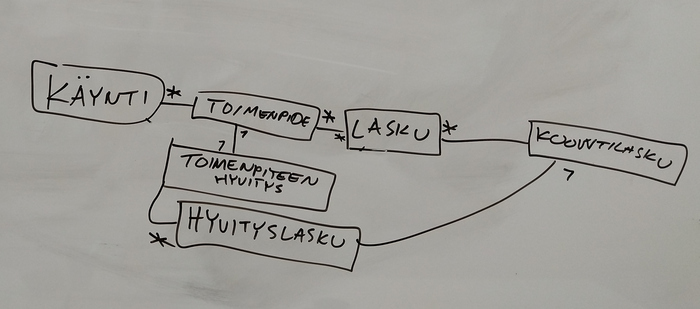
\includegraphics{illustration/malli1.jpg}
\caption{\label{malli1} Ensimmäinen malli}
\end{figure}

Tämän mallin sisältävän ohjelmistoprototyypin toteuttamiseen kului kaksi
viikkoa, ja näin iteraatio oli prosessin pisin. Myöhemmät iteraatiot
kestivät noin viikon. Kulunutta aikaa selittää, että rakensin
prototyypin puhtaalta pöydältä, jolloin aikaa kului myös sovelluksen
pohjan pystyttämiseen.

Ensimmäisessä iteraatiossa syntynyt ohjelmisto ei malliltaan täysin
vastannut tätä ensimmäisen kokouksen piirrosta. Yksinkertaisuuden vuoksi
oletin, että käynnillä on aina vakiohintainen toimenpide, jolloin
Toimenpide-olio jäi mallista pois. Tehdessä huomasin myös, että
koontilaskun ja hyvityslaskun välille ei tarvita mitään suoranaista
yhteyttä. Riittää, että käynti on yhdistetty näihin molempiin.

\hypertarget{iteraatio-2-malli-syvenee}{%
\subsection{Iteraatio 2: malli
syvenee}\label{iteraatio-2-malli-syvenee}}

Iteraation aloittavassa kokouksessa kävimme läpi syntyneen
ohjelmistoprototyypin. Läpikäynnin jälkeen olin hieman epävarma, miten
tapaamista tulisi jatkaa. Päätin ottaa puheeksi minua koko viikon ajan
vaivanneen käyntien ja laskujen läheisen kytköksen. Ohjelmoidessa tuntui
väärältä ja kömpelöltä, että käynti lisätään suoraan laskulle ja vielä
hyvityslaskullekin.

Pyysin Lauraa kertomaan enemmän siitä, mitä käynnin laskuttaminen
oikeastaan tarkoittaa, ja hän kuvasi, millaisissa tilanteissa laskuja
voidaan luoda. Huomioni kiinnittyi puheessa esiintyneeseen termiin
\textbf{Laskutusperuste}. Tämä tuntui valtavan kiinnostavalta, ja Laura
avasi asiaa tarkemmin. Kun laskulle lisätään laskutettavia asioita,
täytyy siihen olla jokin peruste.

Käytimme tapaamisen loppuosan tämän idean kehittelemiseen. Päädyimme
ajatukseen, jossa laskulle lisätään käynnin sijasta palvelurivi, joka
viittaa käyntiin. Tapaamisen jälkeisen viikon kehitystyötä ohjasi nyt
uusi ajattelutapa: käyntiä sinänsä ei liitetä laskuun, vaan käynti
laskutetaan, mikäli laskutusperuste täyttyy.

\begin{figure}
\centering
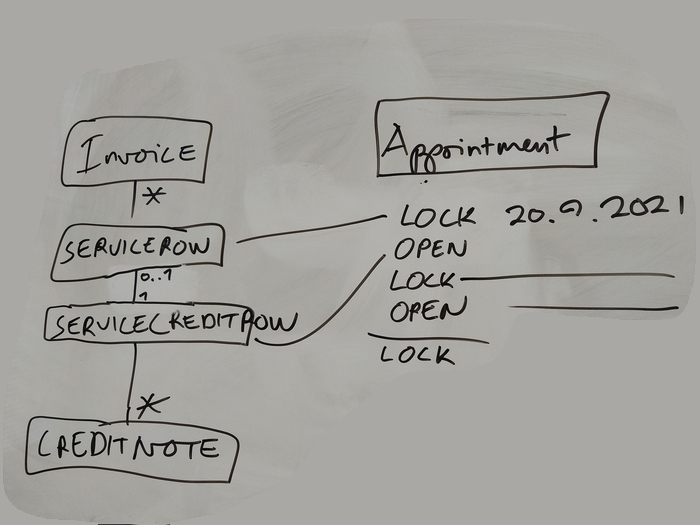
\includegraphics{illustration/malli2.jpg}
\caption{\label{malli2}Toinen malli}
\end{figure}

Yksi toisen tapaamisen aikana syntyneistä malleista on esitetty kuvassa
\ref{malli2}. Siinä laskulle liitetään palvelurivi, joka vastaa
yksittäistä hoitokäyntiä. Mikäli käynti hyvitetään, palveluriviä vastaa
hyvityslaskuun kiinnitetty hyvitysrivi.

Kuvan laidassa näkyy myös hahmotelma siitä, miten käynnin voisi
hyvittämisen jälkeen laskuttaa uudelleen. Sarja monimutkaisia
lukitusoperaatioita tuntui Laurasta jo piirtämisen yhteydessä hankalalta
ymmärtää. On myös kuvaavaa, että pidimme tapaamisen aikana tätä
syntynyttä mallia puutteellisena, ja kehitimme siitä mielestämme
paremman version.

Mallin toteuttamisessa kesti vajaat neljä päivää. Jotta uusi ajatus
palvelurivistä oli mahdollista lisätä koodiin, täytyi olemassaolevaa
ohjelmaa aluksi refaktoroida voimakkaasti. Aiemmin suoraan laskulle
kytkettyyn käyntiin piti sijoittaa sisälle palveluriviä kuvaava olio, ja
lasku muuttaa koostumaan näistä. Käynnin ja hyvityslaskun välinen kytkös
piti katkaista, ja tilalle rakentaa kytkös laskurivin ja hyvitysrivin
välille.

Koodin refaktoroimisessa kului aluksi päivä, ja sen jälkeen uuden,
palvelurivejä ja hyvitysrivejä käsittelevän koodin luomiseen kaksi
päivää.

Perjantaihin tultaessa olin refaktoroinut prototyyppiohjelmaa ja sen
jälkeen käyttänyt kolme päivää ensimmäisen käyttäjätarinan parissa.
Vaikutti, että aikataulu pettää, eikä mitään tule valmiiksi maanantaille
sovittuun seuraavaan tapaamiseen.

Yllättäen perjantaina puolen päivän jälkeen kaikki yksikkötestit menivät
läpi, käyttäjätarina valmistui, ja ohjelmistoprototyypin toiminnassa
tuntui tapahtuvan laadullinen hyppäys. Loppujen kahden käyttäjätarinan
toteuttaminen onnistui kahdessa tunnissa, ja vaati vain joitain rivejä
koodia. \Glsentryname{domainmodel} oli kehittynyt paremmaksi.

Ohjelmoidessa syntynyt tietomalli sisälsi samat asiat, joista
kokouksessa oli puhuttu, mutta niiden suhteet olivat toisenlaiset. Olin
tuottanut ominaisuudet yksikkötesti yksikkötestiltä, ja tämä malli oli
yksinkertaisin, jolla kaikki testit menivät läpi. Malli on esitetty
kuvassa \ref{finalmodel1}

\begin{figure}
\centering
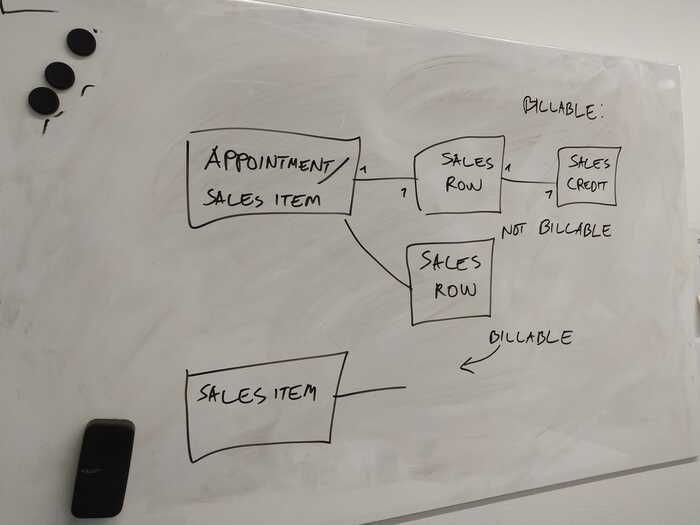
\includegraphics{illustration/final-idea-1.jpg}
\caption{\label{finalmodel1} Kuva, jossa käyntiin kytkeytyy palvelurivi
ja palveluriviin hyvitysrivi}
\end{figure}

\hypertarget{iteraatio-3-malli-osoittaa-joustavuutensa}{%
\subsection{Iteraatio 3: malli osoittaa
joustavuutensa}\label{iteraatio-3-malli-osoittaa-joustavuutensa}}

Kolmannen iteraation aluksi pidimme jälleen suunnittelukokouksen. Tämän
tapaamisen keskeisimpänä ongelmana oli, miten jo kertaalleen laskutettu
ja hyvitetty käynti voidaan laskuttaa uudelleen.

Yritimme piirtää monenlaisia erilaisia malleja ja diagrammeja, mutta
mikään niistä ei tuntunut osuvalta. Tämä tapaaminen oli tunnelmaltaan
kaikista tapaamisista jähmein. Kun kommunikaatio ei sujunut, myöskin
malli kehittyi kehnosti.

Laadimme tapaamisen lopuksi kuitenkin joukon käyttäjätarinoita, jotka
tähtäsivät tavoitteeseemme, hyvitetyn käynnin uudelleenlaskuttamiseen.

Aloitin myös tämän viikon ohjelmointityön samantapaisella mallin
refaktoroinnilla kuin edellisen. Tällä kertaa se oli suppeampi, koska
uusia ajatuksia oli vähemmän.

Ohjelmoidessa yllätyin: sain rakennettua yhdessä päivässä ominaisuuden,
jossa kertaalleen laskutettu ja hyvitetty käynti voidaan laskuttaa
uudelleen. Käytännössä riitti, että muutin käynnillä olevan viittauksen
palveluriviin listamuotoiseksi. Nyt käyntiin oli mahdollista kytkeä
yhden sijasta monta eri palveluriviä, jolloin uudelleenlaskutus
onnistui. Palvelurivien, ja niihin kytkeytyvien hyvitysrivien suhteista
oli helppo rakentaa säännöt sille, onko käynti laskutettavissa vai ei.

Tämä listamuoto on esitetty kuvassa \ref{finalmodel1}. Siinä
tarkastellaan palvelurivien listan viimeisintä jäsentä, ja tällä
perusteella arvioidaan, onko käynti laskutettavissa vai ei.

Kolmas iteraatio oli iteraatioista lyhin, ja se kesti vain noin neljä
päivää.

\hypertarget{iteraatio-4-piilossa-ollut-kuxe4site-luxf6ytyy}{%
\subsection{Iteraatio 4: piilossa ollut käsite
löytyy}\label{iteraatio-4-piilossa-ollut-kuxe4site-luxf6ytyy}}

Neljännen tapaamisen keskeinen ongelma oli, että käynti tuntui olevan
edelleen liian vahvasti kytketty laskuun. Yksittäistä käyntiä vastasi
yksi palvelurivi. Tämä käy ongelmalliseksi, mikäli käynti halutaan jakaa
kahdelle maksajalle. Jo ensimmäisessä tapaamisessa oli käynyt selväksi,
että ainut siisti tapa jakaa käynti kahdelle maksajalle on tehdä kaksi
erillistä laskua. Käyntiin kytkettyä palveluriviä ei kuitenkaan voi
lisätä molemmille laskuille.

Vaikutti siltä, että käynnin ja laskun välistä puuttui edelleen jokin
käsite. Olin keskustellut aiemmin viikolla laskutuksen kanssa
työskennelleen tiimikaverini kanssa, ja hän kiinnitti huomiota siihen,
että laskuille laitettiin ``palvelurivejä''. Hän oli itse käyttänyt
omissa malleissaan ``myyntiä''.

Nyt muistin tämän keskustelun, ja ehdotin sen pohjalta, että
laskutuksessa ei käsiteltäisikään suoraan käyntejä vaan palvelumyyntiä.
Laura totesi, että kaikki laskuille laitettava on lopulta myyntiä -
ikäänkuin se olisi ollut itsestäänselvyys! Ohjelmoijalle tämä oivallus
oli kuitenkin uusi tieto, ja se avasi täysin uuden näkökulman
laskutukseen.

Loimme kokouksessa mallin, jossa Käynti muunnetaan myynniksi eli
SalesItem-olioksi. Nyt käynneistä ei tarvitse välittää lainkaan laskuja
käsiteltäessä. SalesItem puolestaan voidaan jakaa maksajille
suunnatuiksi osuuksiksi, SalesShareiksi, ja yksittäisellä laskulla on
SalesShareen kytketty SalesRow. Malli on esitetty kuvassa \ref{malli3}

\begin{figure}
\centering
\includegraphics{illustration/malli4.jpg}
\caption{\label{malli3}Kolmas malli}
\end{figure}

Kokouksen jälkeen minua odotti jälleen refaktorointityö, joka oli
projektin suurin. Arvioni on, että käynnin perinpohjainen irrottaminen
koko laskutuslogiikasta ja kahden uuden käsitteen laittaminen näiden
väliin olivat keskeisiä syitä sille, miksi muutostyö oli niin työläs.

Uusien ominaisuuksien toteuttaminen refaktoroinnin jälkeen oli
suoraviivaista, ja tuloksena syntyi ohjelma, joka pääsi alkuperäiseen
tavoitteeseensa, jaetun käynnin hyvittämiseen ja uudelleen
laskuttamiseen.

\hypertarget{huomioita-prosessista}{%
\section{Huomioita prosessista}\label{huomioita-prosessista}}

Mallia kehittäessä vaadittujen voimakkaiden refaktorointijaksojen määrä
yllätti. Ennalta kirjallisuudesta luettuna ei refaktoroinnin määrää
ollut helppo hahmottaa. Omakohtainen tekeminen paljasti, miten
oleellinen osa \glslink{ddd}{Sovellusaluevetoista suunnittelua}
refaktorointien tekeminen on.

Refaktoroiminen ei ole tässä tyylissä pelkästään tekninen keino pitää
koodia siistinä, vaan strateginen väline, jonka avulla mallia
parannetaan ja \glslink{ubilang}{kaikenkattavaa kieltä} kehitetään.

Toinen keskeinen keino kaikenkattavan kielen kehittämiseen tässä
prosessissa oli suunnittelutapaamistemme kielen tarkka seuraaminen.
Pyrin nappaamaan Lauran kanssa käydyistä keskusteluista termejä, joita
käytimme, ja etenkin termejä, joita Laura käytti.

Eric Evans mainitsee, että \glsdisp{ubilang}{kaikenkattavan kielen}
rakentamisessa oleellista on löytää sanat, joita alan asiantuntijat
käyttävät.

GraphQL-skeemat tuntuivat heijastavan todella osuvasti rakentamiamme
käsitekarttoja. Useimmiten oli mahdollista siirtää rakentamamme
käsitteiden verkko sellaisenaan GraphQL-skeeman sisälle. Tämä myös
tarkoitti, että palvelinohjelman ja asiakasohjelman välinen rajapinta
sai ensimmäisenä kyvyt uuden käsitekartan version käsittelemiseen.
